\documentclass[12pt,epsf,psfig,graphicx]{article}             

% \documentstyle[bookman,epsf]{article}             
\textwidth = 6.5in
\textheight = 9.05in
\topmargin 0.0in
\oddsidemargin 0.0in
\evensidemargin 0.0in

\usepackage[T1]{fontenc}
\usepackage{mathptmx}
\usepackage{graphicx}

% set it so that subsubsections have numbers and they
% are displayed in the TOC (maybe hard to read, might want to disable)

\setcounter{secnumdepth}{3}
\setcounter{tocdepth}{3}

% define widow protection 
        
\def\widow#1{\vskip #1\vbadness10000\penalty-200\vskip-#1}

% define a little section heading that doesn't go with any number

\def\littlesection#1{
\widow{2cm}
\vskip 0.5cm
\noindent{\bf #1}
\vskip 0.1cm
\noindent
}

% A paraphrase mode that makes it easy to see the stuff that shouldn't
% stay in for the final proposal

\newdimen\tmpdim
\long\def\paraphrase#1{{\parskip=0pt\hfil\break
\tmpdim=\hsize\advance\tmpdim by -15pt\noindent%
\hbox to \hsize
{\vrule\hskip 3pt\vrule\hfil\hbox to \tmpdim{\vbox{\hsize=\tmpdim
\def\par{\leavevmode\endgraf}
\obeyspaces \obeylines 
\let\par=\endgraf
\bf #1}}}}}

\renewcommand{\baselinestretch}{1.2}    % must go before the begin of doc
\newtheorem{principle}{Principle}
\newtheorem{definition}{Definition}
% go with the way that CC sets the margins

\begin{document}

% handle widows appropriately
\def\widow#1{\vskip #1\vbadness10000\penalty-200\vskip-#1}

\begin{center}

CS290: Principles of Software Development \\
Examination Two \\

\end{center}

\noindent Answer the five questions that are listed on the following pages.  You must provide answers to these questions
on a separate sheet of paper.  Please develop responses that clearly express your ideas in the most succinct manner
possible.  You are not permitted to complete this examination in conjunction with any of your classmates.  Furthermore,
you cannot consult any outside references during this examination.  If you have questions concerning the following
problems, then please visit my office during the examination period.  If you leave the classroom to take the exam, then
you are responsible for checking the white board for status updates.

% \noindent Answer the five questions that are listed below.  You must provide answers to these questions on a separate
% sheet of paper.  Please develop responses that clearly express your ideas in the most succinct manner possible.  You are
% not permitted to complete this examination in conjunction with any of your classmates.  Furthermore, you cannot consult
% any outside references during this examination.  If you have questions concerning the problems that are listed below,
% then please visit my office during the examination period.  If you leave the classroom to take the exam, then you are
% responsible for checking the white board for status updates.
% 
\begin{enumerate}

\item ({\bf 10 Points}) Requirements elicitation and analysis is an important part of the overall software life cycle.
	Answer the following questions about software requirements.

\begin{enumerate}

	\item ({\bf 2 Points}) What is a software requirement? Why is it important to define the requirements of a software
		application before starting to implement it?

	\item ({\bf 4 Points}) Please define and give at least one example of each type of requirement.

		\begin{enumerate}
			\item Functional requirement
			\item Non-functional requirement
			\item Design constraint
			\item Process constraint
		\end{enumerate}

	\item ({\bf 4 Points}) There are at least eight ``requirements'' for software requirements.  Please name and define
		four of the eight requirements; state the importance of each of these.


% What is a software requirement?

% \item ({\bf 6 Points}) Sommerville argues that there are six
%   requirements to which all requirements should adhere.  What are
%   these six requirements?
% 

% \item ({\bf 3 Points}) Software engineers commonly organize
%   requirements into the following three categories: {\em functional},
%   {\em non-functional}, and {\em domain}.  Please provide a definition
%   and an example of these three types of requirements.
% 
\end{enumerate}

\newpage

\begin{figure}[t]
	\centering
	\begin{tabular}{c c}
		\begin{minipage}{3.4in} 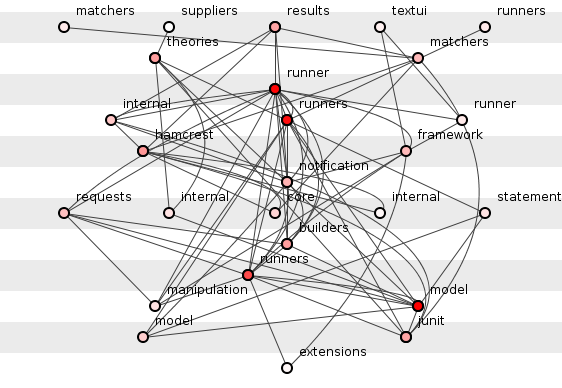
\includegraphics[width=3in]{45.png} \vspace*{-.2in} \begin{center}(a)\end{center} \end{minipage} & 
		\begin{minipage}{3.4in} 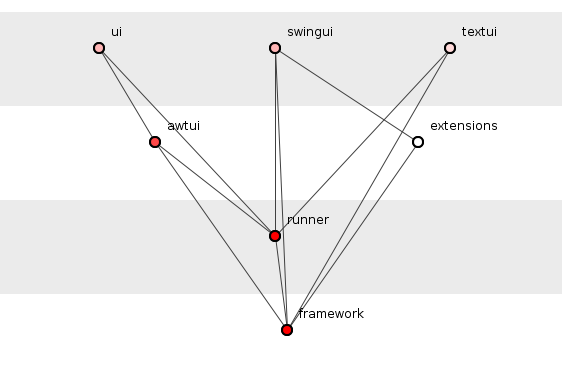
\includegraphics[width=3in]{37.png} \vspace*{-.2in} \begin{center}(b)\end{center} \end{minipage}
 	\end{tabular}
	\caption{The Evolving Architecture of the JUnit Test Automation Framework.}
	\label{fig:junit}
\end{figure}

\item ({\bf 10 Points}) An engineer must be able to capture and use the requirements for a system.  Answer the following
	questions about requirements elicitation and software architecture.

\begin{enumerate}

\item ({\bf 3 Points}) Francis Bacon said that ``truth emerges more readily from error than confusion.''  What does this
	quote mean?  How does it apply to the task of requirements elicitation and analysis? Please support your response to
	this question with a concrete example from either a laboratory assignment or the final project.

\item ({\bf 3 Points}) What is the architecture of a software system? How is it distinct from the requirements? How is
	it different than the design of the same software system? 

\item ({\bf 4 Points}) Figure~\ref{fig:junit}(a) and (b) give two diagrams that depict the software
	architecture of the JUnit testing framework.  Answer the following questions about these diagrams.

	\begin{enumerate}
		\item One of these diagrams explains an early stage of JUnit's implementation while the other depicts late-stage
			structure.  Which one is which? How do you know?

		\item Why do you think the early- and late-stage diagrams look the way that they do?
	\end{enumerate}

% \item ({\bf 4 Points}) The process for capturing the requirements of a
%   software system normally includes four distinct phases.  Draw a
%   diagram that shows each of these phases and indicates how a software
%   engineer can proceed through them.  In your diagram, a square or a
%   rectangle should denote a phase and a directed edge should show a
%   possible way to follow from one phase to the next.
% 

% \item ({\bf 2 Points}) Hamlet and Maybee argue that requirements
%   should be {\em non-prescriptive}.  What does it mean if a
%   requirement has this characteristic?  After defining this term,
%   please give an example of a non-prescriptive requirement.
% 
\end{enumerate}

\newpage

\item ({\bf 10 Points}) Research in software architectures has flourished in recent years.  Answer the following
	questions about software architectures by providing a response for each part.

\begin{enumerate}

% \item ({\bf 2 Points}) Define the term software architecture.  Discuss some of the advantages to explicitly designing
% and documenting a software architecture.
% 
\item ({\bf 4 Points}) The shared repository (or tuple space or blackboard model is one example of a
	software architecture.  Please draw a diagram that explains how this architecture works.  What is one strength and
	one weakness of this architecture?

\item ({\bf 4 Points}) The pipe and filter is another example of a software architecture.  In the context of this
	architecture, what is the meaning of the terms pipe and filter?  Your response to this question should
	also furnish an example of a pipe and filter architecture in the context of the GNU/Linux command line.

\item ({\bf 2 Points}) One benefit of the pipe and filter architecture is that it supports the analysis of throughput
	and response time.  Draw and explain two graphs that depict the relationship between throughput and 	response
	time and the length of the pipe and filter chain.  The first graph should have the label ``throughput'' on the
	vertical axis and ``length of the pipe and filter chain'' on the horizontal while the second should have ``response
	time'' on the vertical and ``length of the pipe and filter chain'' on the horizontal.

\end{enumerate}

\newpage

% Note: something about the visitor design pattern.

\item ({\bf 10 Points}) It is essential for a software system to have a design that is easy to understand and implement.
	Answer the following questions about the design of software.

\begin{enumerate}

\item ({\bf 3 Points}) What does it mean if two modules in a system are tightly coupled? Loosely coupled? What is the
	difference between control and data coupling between modules?

% Afferent Couplings (Ca)
% The number of other packages that depend upon classes within the package is an indicator of the package's responsibility.
% 
% Efferent Couplings (Ce)
% The number of other packages that the classes in the package depend upon is an indicator of the package's independence.
% 

\item ({\bf 3 Points}) The packages within a Java program can exhibit either afferent or efferent couplings.  What is
	the meaning of these two types of coupling? Your response to this question should furnish a diagram to illustrate
	each type of coupling.   

\item ({\bf 4 Points}) The unified modeling language (UML) provides diagrams that visualize both static and dynamic
	views of a software system.  After explaining the terms static and dynamic view and furnishing and example of each,
	your response to this question should discuss the similarities and differences between these two types of views.

\end{enumerate}

\newpage

\item ({\bf 10 Points}) When it comes to developing high quality software applications, it is important to properly
	complete all of the phases of the software life cycle.  Answer the following questions about the life cycle that you
	can follow to engineer software.

\begin{enumerate}

\item ({\bf 4 Points}) Suppose that you are part of a development team that is responsible for implementing a compiler
	for the Java programming language.  The manager of your team asks you to fully implement array-bounds checking
	in your compiler.  After defining what this term means, explain whether or not this requirement is feasible.

\item ({\bf 2 Points}) After conducting an empirical investigation of software errors, Basili and Perricone draw the
	following conclusion: ``48 percent of faults observed in a medium-scale software project were attributed to
	incorrect or misinterpreted functional specifications or requirements.''  In your opinion, why is this the case?

\item ({\bf 2 Points}) When specifying and designing a software, it is often useful to specify a method's preconditions
	and postconditions. What is the meaning of these two terms?

\item ({\bf 2 Points}) The Visitor design pattern requires the use of the {\tt visit} and {\tt accept} methods.  What is
	the purpose of these methods? During the execution of a program that uses the Visitor design pattern, in what order
	are these methods called?



% \item ({\bf 4 Points}) It is important to develop ways to rate
%   the quality of a requirements document since the individual
%   requirements are used by the designers, implementers, and
%   testers throughout the remainder of the lifecycle.  Pfleeger
%   and Atlee outline the following scale for evaluating a
%   requirement:
% 
% \renewcommand{\labelitemi}{$-$}
% 
%           \begin{itemize}
% 
%           \item 1 - You (the designer) understand this requirement
%             completely, you have designed from similar requirements in
%             the past, and you should have no trouble developing a
%             design from this requirement.
% 
%           \item 2 - There are elements of this requirement that are
%             new to you, but they are not radically different from
%             requirements that you have successfully designed from in
%             the past.
% 
%           \item 3 - There are elements of this requirements that are
%             very different from requirements that you have designed
%             from in the past, but you understand the requirement and
%             you think that you can develop a good design from it.
% 
%           \item 4 - There are parts of this requirement that you do
%             not understand, and you are not sure that you can develop
%             a good design.
% 
%           \item 5 - You do not understand this requirement at all, and
%             you cannot develop a design for it.
% 
%           \end{itemize}
% 
%           Using this rating scheme, it is possible to determine
%           whether or not a software development team should start to
%           design and implement the system.  As part of your response
%           to this question, please draw two {\em histograms} where the
%           vertical axis is the {\em number} of requirements in each of
%           the above categories and the horizontal axis gives the {\em
%             categories} in numerically increasing order (i.e., 1 to
%           5).  One of the histograms must represent a system that is
%           ready to leave the requirements elicitation and analysis
%           phase and the other should reveal that it is not advisable
%           to start the architecture and design phase.  Your response
%           should clearly explain why you created the histograms in
%           this way.
% 
\end{enumerate}

\end{enumerate}

\end{document}



